\documentclass[unicode,pdfcover]{./scut_thesis/scutthesis}

\usepackage[unicode=false,bookmarks=true,bookmarksnumbered=true,bookmarksopen=false,
    breaklinks=false,pdfborder={0 0 1},backref=false,colorlinks=true]
{hyperref}

\hypersetup{pdftitle={小型涵道式无人机气动参数辨识和近地面抗扰控制},
    pdfauthor={崔启权},
    pdfsubject={华南理工大学硕士学位论文},
    pdfkeywords={关键字1, 关键字2},
    linkcolor=blue, anchorcolor=black, citecolor=olive, filecolor=magenta, menucolor=red, urlcolor=magenta, pdfstartview=FitH}

\begin{document}


\includepdf[pages=-]{"scut_thesis/thesis_cover.pdf"}
\frontmatter

\begin{abstractCN}
    本文用于测试scutthese.cls的使用，主要包括xelatex是否正常可调用，中文字体是否显示之前，pdf标签是否正确显示。
    1、介绍涵道式无人机
    2、涵道式无人机面临的困境
    3、介绍本文作出的贡献
    针对各个细分问题给出解决方案
    4、做出总结
\end{abstractCN}
\keywordsCN{飞行器；涵道风扇式无人机}

\begin{abstractEN}
    English abstract
\end{abstractEN}
\keywordsEN{\LaTeX{};  Typesetting; Paper}



\tableofcontents{}

\listoftables


\listoffigures



\chapterx{主要符号对照表}

【本节论文规范为可选，如果你的论文没有相关内容那么去除这一节；如果有，则删除这一行注释。】

\begin{table}
    \centering{}%
    \begin{tabular}{l>{\centering}p{2.5cm}l}
        $Q$ - 系统最大取向数            &  & $d_{MC}$ - 网格常数(m)\tabularnewline
        $\varepsilon_{e}$ - 弹性应变 &  & $k$ - Blozmann常数$\left(J/K\right)$\tabularnewline
                                 &  & \tabularnewline
                                 &  & \tabularnewline
                                 &  & \tabularnewline
    \end{tabular}
\end{table}

\mainmatter

% 绪论
\chapter{绪论}
无人驾驶航空器（Unmanned Aerial Vehicle, UAV）的快速发展正在深刻重塑现代社会的生产生活方式。作为低空经济（Low-Altitude Economy）的核心载体，无人机凭借其灵活性、便捷性和可扩展性，在军事侦察、精准农业、工业巡检、城市物流等众多领域展现出巨大的应用潜力。旋翼无人机相较于固定翼飞行器，其垂直起降和悬停能力使其在执行定点、精准和详查任务时独具优势，填补了有人驾驶航空器在复杂环境下的作业空白。

近年来，低空经济作为战略性新兴产业，正加速从“飞起来”向“用起来”跃升。据预测，2025年我国低空经济市场规模将达到1.5万亿元，2030年有望突破2万亿元。在军事领域，无人机已成为现代战争中情报获取、目标监视乃至精确打击的关键装备；在农业领域，农用无人机突破地形与人力限制，让播种、植保、监测从地面延伸至低空；在工业领域，无人机广泛应用于电力巡检、油气管道监测、光伏面板清洁等作业场景，显著提升了运维效率；在运输领域，无人机物流正从试点走向常态——从城市上空的“分钟级配送”到山区乡村的“最后一公里”，低空物流正在改变传统物流格局，医疗样本的空中转运更成为守护生命的快速通道。2026年5月即将实施的《民用无人驾驶航空器实名登记和激活要求》与《民用无人驾驶航空器系统运行识别规范》，标志着我国无人机产业正从“野蛮生长”走向“规范提质”，为低空经济的健康可持续发展奠定了制度基础。

在众多无人机技术路线中，涵道式无人机（Ducted Fan UAV）因其独特的结构设计和优异的气动性能，日益受到学术界和工业界的广泛关注\cite{renxiaolu}\cite{xuchang}。涵道风扇（Ducted Fan）是指在螺旋桨风扇外围设置涵道（导管）的一种推进装置，其工作原理与孤立螺旋桨有本质区别。

从结构特点来看，涵道式无人机具备以下几方面突出优势：

第一，安全性高。涵道将旋翼完全或大部分环括于内部，能有效避免裸露旋翼割伤人员和碰撞障碍物的事故发生。这一特性使涵道式无人机特别适合在狭小空间、近人环境以及城市复杂地形中作业。例如，以色列Urban Aeronautics公司开发的Cormorant（又称AirMule）无人机，采用涵道风扇技术，可在建筑物密集区域、陡峭山地等传统直升机难以进入的环境执行搜救和物资投送任务，其旋翼内置设计不仅提高了安全性，也显著降低了气动噪声。中国航天科工二院研发的微小型涵道风扇无人机，外表采用柔软发泡材料包裹，进一步提升了防撞性能，完全满足近地/近人场景的安全需求。

第二，气动效率高。涵道的存在改变了风扇的气动工作环境：一方面，涵道限制了叶尖涡流的形成和发展，减少了诱导阻力，从而降低能量损失；另一方面，涵道入口的合理设计可改善进气条件。研究表明，与同等直径的孤立螺旋桨相比，涵道风扇能够产生更高的推力性能、更高的推进效率和更低的噪声特性\cite{Numerical_and_Experimental_Analyses_of_the_Ducted_Fan}。通过将螺旋桨封闭在涵道内，不仅可以降低裸露旋翼带来的风险，还能通过减小叶尖损失和优化气流组织来改善气动性能\cite{Aerodynamic_performance_assessment_of_a_ducted_fan_UAV}。近期研究还表明，针对边界层吸入（Boundary Layer Ingestion, BLI）进气条件，通过在涵道唇口设计鼓包等流动控制方法，可有效改善进气畸变，降低气动损失\cite{wangshuo}。

第三，具备垂直起降能力且结构紧凑。涵道式无人机继承了旋翼飞行器垂直起降和悬停的优点，能够在无跑道条件下起降，适用于舰载、山地、城市峡谷等复杂环境。同时，涵道结构使整机布局更为紧凑，体积小巧，便于携带和收纳。北京猎鹰无人机开发的LY-20涵道式油电混合无人机，兼具电动多旋翼的精准悬停能力和油动无人机的长航时优势，可广泛应用于消防侦察、公安巡逻、光伏巡检等领域。涵道向下的强风还可用于清洁太阳能电池板表面灰尘，在光伏产业中具有独特应用价值。

涵道式无人机以其安全可靠、气动高效、垂直起降和结构紧凑等综合优势，正成为无人机技术研究的重要方向之一。随着低空经济应用场景的持续拓展，涵道式无人机在人员搜救、复杂环境侦查、管道巡检、城市空中交通等领域的应用前景将更加广阔。深入开展涵道式无人机气动设计、飞行控制与系统集成研究，对于推动我国无人机技术自主创新、抢占低空经济制高点具有重要的理论意义和工程价值。



Tex排版\cite{knuth1986thetexbook}是由Knuth最早发明，后来人们对其扩展了大量宏包以增强其功能，而且设计了多种不同的Tex专业引擎，其中内置了许多常用的Tex宏包，如\LaTeX{}；内核不同的新TEX引擎，如XeTex（包含LaTex宏包的称为XeLaTex），它支持支持UTF-8文档编码而以pdf格式输出。

XeTex引擎使用xeCJK宏包支持中文排版\cite{goossens1994thelatex}，大大方便了中日韩语言用户排名。我们自定义了scutthesis.cls模板库，它是基于latex/base/book.cls进行文章结构布局,并调用了xelatex/xecjk/xeCJK.sty宏包，以UTF-8方式支持中文显示。scutthesis.cls模板库是一套“华南理工大学博士学位论文”模板。见\ref{fig:aircraft}。

\begin{figure}
    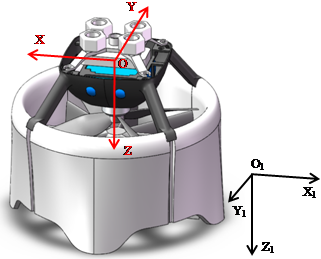
\includegraphics[scale=0.5]{figure/body1.png}
    \caption{\label{fig:aircraft}涵道式无人机结构图}
\end{figure}

this is a book! beautiful book!和一个文章。\cite{knuth1986thetexbook}
测试中文section的标题名，中文文献引用\cite{Krasnogor2004e, wang_model_2009}.


\section{小型涵道式无人机的系统构成与建模}

\section{展望与总结}


\backmatter

\bibliographystyle{scut_thesis/scutthesis}
\bibliography{refrence}

\appendix{附录}
\section{Ubuntu Linux系统下中文字体的安装}
\label{sec:ubuntuzhfont}
整个过程分为两部分：得到中文字体文件和安装设置。

常用中文字体有三套：

1. winfonts（微软的六种中易字体，包括宋体、黑体、楷书、仿宋、隶书、幼圆），

2. adobefonts（Adobe 的四套字体，包括 Adobe Song Std、Adobe Heiti Std、Adobe
Fangsong Std、Adobe Kaiti Std）

3. Ubuntu开源的文泉字体
CTex宏库默认支持winfonts和adboefonts。因此要在linux系统下使用Ctex宏库最好是安装这些字库之一。

\section{Texlive的安装}

\label{sec:texlive_install}

Texlive是TEX的一个集成发行包，相关介绍见http://tug.org/texlive/doc/texlive-zh-cn/。其主要过程包括：预设置、下载安装和测试调用。建议用GUI方式安装：

sudo apt-get install perl-tk

到http://tug.org/texlive/acquire-netinstall.html页面下载 install-tl在线安装前端程序.


\chapterx{攻读博士学位期间取得的研究成果}

已发表（包括已接受待发表）的论文，以及已投稿、或已成文打算投稿、或拟成文投稿的论文情况（只填写与学位论文内容相关的部分）：

\begin{longtable}{|>{\centering}m{0.5cm}|>{\centering}m{2.3cm}|>{\centering}m{3.5cm}|>{\centering}m{2.6cm}|>{\centering}m{2cm}|>{\centering}m{1.3cm}|>{\centering}m{0.9cm}|}
    \hline
    序号 & 作者（全体作者，按顺序排列） & 题 目   & 发表或投稿刊物名称、级别 & 发表的卷期、年月、页码 & 相当于学位论文的哪一部分（章、节） & 被索引收录情况\tabularnewline
    \hline
    1  & 作者名            & 论文题目1 & 刊物名          & 发表时间        & 第2章               & SCI\tabularnewline
    \hline
    2  & 作者名            & 论文题目2 & 刊物名          & 发表时间        & 第3章               & SCI\tabularnewline
    \hline
       &                &       &              &             &                   & \tabularnewline
    \hline
       &                &       &              &             &                   & \tabularnewline
    \hline
       &                &       &              &             &                   & \tabularnewline
    \hline
       &                &       &              &             &                   & \tabularnewline
    \hline
\end{longtable}


\chapterx{致谢}

首先感谢国家，感谢党；再感谢导师对我的指导，最后感谢父母亲对我的期望！

同时感谢华工校内外多位同学对该模板的测试和提供的改进。

\begin{minipage}[t]{0.8\columnwidth}%
    \begin{flushright}
        徐顺
        \par\end{flushright}

    \begin{flushright}
        \today
        \par\end{flushright}%
\end{minipage}

\end{document}
